\section{Results and Discussion}
\label{sec:resultsanddiscussion}

Testing and analysis were performed on the design and implementation previously designed. The tests include the Load Cell Sensor testing on the Robot and the Robot Balance System.

\begin{enumerate}[label=\Alph*.]

    \item Characterization Testing of Each Load Cell
    \label{subsec:results-discussion-characterization}

        \hspace*{1em} Calibration testing of the load cell sensors was conducted using five reference masses (50g, 100g, 200g, 500g, and 1000g). The smallest weight (50 grams) was used to determine the gradient coefficient, while the constant was obtained from the tare weight (zero point when the load cell has no load). The resulting data was then used to calculate the error of each load cell by comparing it with the actual mass.

        \begin{table}[h!]
            \centering
            \caption{Characterization Results of Load Cell 1}
            \begin{tabular}{|c|c|c|}
                \hline
                \textbf{Actual Weight (g)} & \textbf{Load Cell 1 Reading (g)} & \textbf{Error (g)} \\
                \hline
                50    & 50    & 0   \\
                100   & 101   & 1   \\
                200   & 202   & 2   \\
                500   & 505   & 5   \\
                1000  & 1004  & 4   \\
                \hline
            \end{tabular}
            \label{tab:Calibration_Load_Cell_1}
        \end{table}

        \begin{table}[h!]
            \centering
            \caption{Characterization Results of Load Cell 2}
            \begin{tabular}{|c|c|c|}
                \hline
                \textbf{Actual Weight (g)} & \textbf{Load Cell 2 Reading (g)} & \textbf{Error (g)} \\
                \hline
                50        & 50        & 0   \\
                100       & 100       & 0   \\
                200       & 200       & 0   \\
                500       & 500       & 0   \\
                1000      & 994       & 6   \\           
                \hline
        \end{tabular}
        \label{tab:Calibration_Load_Cell_2}
        \end{table}

        \begin{table}[h!]
            \centering
            \caption{Characterization Results of Load Cell 3}
            \begin{tabular}{|c|c|c|}
                \hline
                \textbf{Actual Weight (g)} & \textbf{Load Cell 3 Reading (g)} & \textbf{Error (g)} \\
                \hline
                50        & 50        & 0    \\    
                100       & 103       & 3    \\    
                200       & 203       & 3    \\    
                500       & 494       & 6    \\    
                1000      & 981       & 19   \\               
                \hline
        \end{tabular}
        \label{tab:Calibration_Load_Cell_3}
        \end{table}

        \begin{table}[h!]
            \centering
            \caption{Characterization Results of Load Cell 4}
            \begin{tabular}{|c|c|c|}
                \hline
                \textbf{Actual Weight (g)} & \textbf{Load Cell 4 Reading (g)} & \textbf{Error (g)} \\
                \hline
                50        & 50        & 0   \\     
                100       & 97        & 3   \\     
                200       & 204       & 4   \\     
                500       & 500       & 0   \\     
                1000      & 1003      & 3   \\                
                \hline
        \end{tabular}
        \label{tab:Calibration_Load_Cell_4}
        \end{table}
    
        
        \hspace*{1em} The characterization results for each load cell show measurement errors ranging from 0 to 19 grams. These errors are non-linear, indicating that the measurement errors are not constant across each load cell. Nevertheless, a linear equation can still be used to calculate the actual mass from the load cell readings, although it is not entirely accurate.

    \item Pressure Testing on the Footpads
    \label{subsec:results-discussion-pressure}

        \hspace*{1em} This test was conducted to obtain pressure data generated by the right and left feet when subjected to a uniform load. The pressure data generated by the right and left feet can be seen in Table \ref{tab:measurement_weight_left_foot} and Table \ref{tab:measurement_weight_right_foot}.

        \begin{table}[h!]
            \centering
            \caption{Pressure Readings for the Left Foot}
            \begin{tabular}{|c|c|c|}
                \hline
                \textbf{Actual Weight (g)} & \textbf{Reading (g)} & \textbf{Error (g)} \\
                \hline
                50    & 52    & 2   \\
                100   & 110   & 10  \\
                200   & 220   & 20  \\
                300   & 304   & 4   \\
                500   & 512   & 12  \\
                700   & 701   & 1   \\
                1000  & 1050  & 50  \\
                1300  & 1325  & 25  \\
                1500  & 1512  & 12  \\
                1800  & 1788  & 12  \\
                \hline
                \textbf{Average Error (g)} & \multicolumn{2}{c|}{\textbf{14.8}} \\
                \hline
            \end{tabular}
            \label{tab:measurement_weight_left_foot}
        \end{table}

        \begin{table}[h!]
            \centering
            \caption{Pressure Readings for the Right Foot}
            \begin{tabular}{|c|c|c|}
                \hline
                \textbf{Actual Weight (g)} & \textbf{Reading (g)} & \textbf{Error (g)} \\
                \hline
                50    & 46    & 4    \\
                100   & 98    & 2    \\
                200   & 215   & 15   \\
                300   & 325   & 25   \\
                500   & 505   & 5    \\
                700   & 722   & 22   \\
                1000  & 1025  & 25   \\
                1300  & 1347  & 47   \\
                1500  & 1500  & 0    \\
                1800  & 1819  & 19   \\
                \hline
                \textbf{Average Error (g)} & \multicolumn{2}{c|}{\textbf{16.4}} \\
                \hline
            \end{tabular}
            \label{tab:measurement_weight_right_foot}
        \end{table}

        \begin{figure}[h]
            \centering
            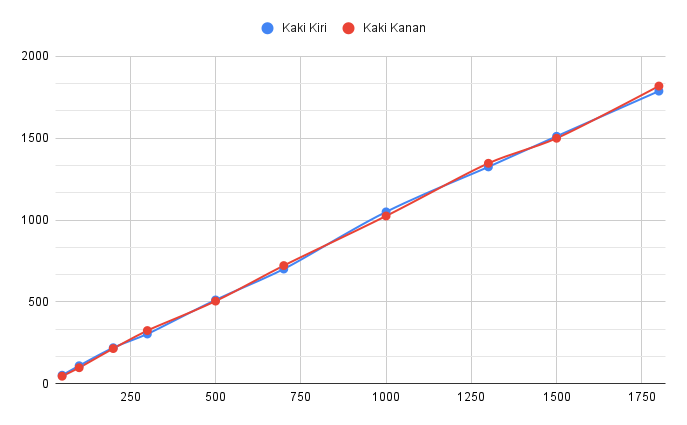
\includegraphics[width=0.4\textwidth]{gambar/chart_tekanan_kaki.png}
            \caption{Graph of the Relationship Between Actual Weight and Load Cell Readings for the Left and Right Feet}
            \label{fig:foot_pressure}
        \end{figure}

        \hspace*{1em} Figure \ref{fig:foot_pressure} shows that the pressure graphs produced by the right and left feet have similar reading values. The pressure measurement results for the left and right feet show that the load cell readings on both feet have errors ranging from 0 to 50 grams. These errors are due to differences in characteristics between the load cells on the left and right feet. 
        
    \item PID Control System Testing
    \label{subsec:results-discussion-pid}

    \hspace*{1em} This test was conducted to analyze the effect of each PID parameter. The results to be analyzed include the impact of PID parameters on system response and the Root Mean Square (RMS) values generated by the system. The testing was performed by lifting either the right or left foot at a 3-degree tilt. The following are the results of the robot balance system testing.

    \begin{table}[h]
        \centering
        \caption{Effect of Parameter $K_p$ on Left Foot Lifting with 3-Degree Tilt}
        \begin{tabular}{|c|c|c|c|c|}
            \hline
            \textbf{PID} & \textbf{Fall} & \textbf{Not Fall} & \textbf{Success} & RMS Error \\
            \hline
            $K_p = 0.00$ & 6 & 0 & 0   \% & 0.7598 \\
            $K_p = 0.05$ & 6 & 0 & 0   \% & 0.7690 \\
            $K_p = 0.10$ & 0 & 6 & 100 \% & 0.7779 \\
            $K_p = 0.15$ & 1 & 5 & 83  \% & 0.8145 \\
            $K_p = 0.20$ & 1 & 5 & 83  \% & 0.8870 \\
            $K_p = 0.25$ & 0 & 6 & 100 \% & 0.8801 \\            
            \hline
        \end{tabular}
        \label{tab:testing_p}
    \end{table}

    \hspace*{1em} The results shown in Table \ref{tab:testing_p} indicate that the optimal $K_p$ parameter value for maintaining robot balance ranges from 0.10 to 0.20. At $K_p = 0.00$ and $K_p = 0.05$, all tests failed, and the robot consistently fell. The $K_p = 0.10$ value shows the best performance with a 100\% success rate in maintaining balance during right and left foot lifting at a 3-degree tilt. Higher $K_p$ values, such as $K_p = 0.25$, show a decline in performance. The Root Mean Square (RMS) results indicate the smallest error at $K_p = 0.10$ with a value of 0.7779, highlighting the importance of setting an appropriate $K_p$ value for robot stability.

    \begin{table}[h]
        \centering
        \caption{Effect of Parameter $K_i$ on Right Foot Lifting with 3-Degree Tilt}
        \begin{tabular}{|c|c|c|c|c|}
            \hline
            \textbf{PID} & \textbf{Fall} & \textbf{Not Fall} & \textbf{Success} & RMS Error \\
            \hline
            $K_p = 0.1, K_i = 0.01$ & 2 & 4 & 66 \%  & 0.9701\\
            $K_p = 0.1, K_i = 0.02$ & 2 & 4 & 66 \%  & 0.8950\\
            $K_p = 0.1, K_i = 0.04$ & 1 & 5 & 83 \%  & 0.9345\\
            $K_p = 0.1, K_i = 0.10$ & 0 & 6 & 100 \% & 0.8471\\
            $K_p = 0.1, K_i = 0.20$ & 0 & 6 & 100 \% & 0.8980\\           
            \hline
        \end{tabular}
        \label{tab:testing_pi}
    \end{table}

    \hspace*{1em} The results shown in Table \ref{tab:testing_pi} indicate that the optimal $K_i$ parameter value for maintaining robot balance ranges from 0.10 to 0.20. At $K_i = 0.01$ and $K_i = 0.02$, the robot failed to maintain balance with a success rate of 66\% to 83\%. Conversely, at $K_i = 0.10$ and $K_i = 0.20$, the robot successfully maintained balance with a 100\% success rate during right and left foot lifting at a 3-degree tilt. The Root Mean Square (RMS) results show the lowest value at $K_i = 0.10$ with 0.8471, while the highest value at $K_i = 0.01$ is 0.9701. The influence of $K_i$ on performance is not very significant, and in some cases, higher $K_i$ values reduce system performance, indicating that the $K_i$ parameter in the PID control for this system is not very critical.

    \begin{table}[h]
        \centering
        \caption{Effect of Parameter $K_d$ on Right Foot Lifting with 3-Degree Tilt}
        \begin{tabular}{|c|c|c|c|c|}
            \hline
            \textbf{PID} & \textbf{Fall} & \textbf{Not Fall} & \textbf{Success} & RMS Error \\
            \hline
            $K_p = 0.1, K_d = 0.005$ & 0 & 6 & 100 \% & 0.7143 \\
            $K_p = 0.1, K_d = 0.010$ & 0 & 6 & 100 \% & 0.7077 \\
            $K_p = 0.1, K_d = 0.020$ & 2 & 4 & 66  \% & 0.7262 \\
            $K_p = 0.1, K_d = 0.050$ & 5 & 1 & 16  \% & 0.7344 \\
            $K_p = 0.1, K_d = 0.100$ & 6 & 0 & 0   \% & 0.9231 \\          
            \hline
        \end{tabular}
        \label{tab:testing_pd}
    \end{table}

    \hspace*{1em} The results shown in Table \ref{tab:testing_pd} indicate that the optimal $K_d$ parameter value for maintaining robot balance ranges from 0.005 to 0.020. At $K_d = 0.005$ and $K_d = 0.010$, the robot successfully maintained balance with a 100\% success rate. However, at $K_d = 0.020$, the success rate decreased to 66\%, and at $K_d = 0.050$, the success rate was only 16\%. At $K_d = 0.100$, the robot consistently fell. The Root Mean Square (RMS) results show the lowest value at $K_d = 0.010$ with 0.7077, while the highest value at $K_d = 0.100$ is 0.9231. The impact of $K_d$ on system performance is quite significant, with higher $K_d$ values reducing system performance.


\end{enumerate}
